\documentclass[a4paper,12pt]{article}

\usepackage[utf8]{inputenc}

\usepackage{graphicx}

\usepackage{geometry}

\usepackage{xcolor}

\usepackage[pdftex]{hyperref}

\usepackage{caption}

\geometry{margin=1in}
 
\title{Modelo Relacional UML da Aplicação Camaar}

\author{
  Silva, Gabriel\\
  \texttt{222005401}
  \and
  Oliveira, Luigi\\
  \texttt{190062894}
  \and
  Ximenes, Pedro\\
  \texttt{200026071}
  \and
  Junior, Weldo\\
  \texttt{222014133}
}

\date{}

\begin{document}
 
\maketitle

\section*{Introdução}

A aplicação \textbf{Camaar} é um sistema desenvolvido em \textbf{\textit{Rails Full-Stack}}, que será utilizado para fins educacionais de aprendizado como projeto final da disciplina de \textbf{Engenharia de Software} da \textbf{UnB} (Universidade de Brasília) do período de 2025.1. 

Essa aplicação permite a gestão de formulários relacionados à turmas/disciplinas da UnB, esses formulários poderão ser respondidos por professores e alunos. Este relatório apresenta o modelo relacional UML simplificado para a aplicação, descrevendo suas principais entidades, atributos e relacionamentos.
 
 
\section*{Entidades Principais}
 
\subsection*{1. Formularios}

\begin{itemize}

    \item \textbf{id}: Identificador único (\textit{chave primária}).

    \item \textbf{template\_id}: Referência ao template do formulário (\textit{Template.id}).

    \item \textbf{destinatario\_cargo}: Cargo ao qual será destinado o formulário (ex: aluno, professor) (\textit{Ocupacao}).

    \item \textbf{status\_ativo}: se o formulário ainda está disponível para responder (\textit{booleano}).

    \item \textbf{classe\_id}: Referência a matérias (\textit{Materia.id}).

\end{itemize}

Relacionamento: Um formulário está associado a uma matéria e a um template. Um formulário pode ter várias respostas. 

\subsection*{2. Respostas}

\begin{itemize}

    \item \textbf{id}: Identificador único (\textit{chave primária}).

    \item \textbf{resposta\_discursiva}: Respostas discursiva de um questão (\textit{str}).

    \item \textbf{resposta\_multipla\_escolha}: Chave estrangeira associada ao usuário (\textit{int}).

    \item \textbf{questao\_id}: Referência a questoes (\textit{Questoes.id}).

    \item \textbf{formulario\_id}: Referência a formularios (\textit{Formularios.id}).
    
    \item \textbf{usuario\_id}: Referência a usuarios (\textit{Usuarios.id}).

\end{itemize}

Relacionamento: Várias respostas estão associadas a um formulário. Cada resposta está ligada a um usuário.

\subsection*{3. Questoes (Questões)}

\begin{itemize}

    \item \textbf{id}: Identificador único (\textit{chave primária}).

    \item \textbf{tipo\_questao}: Tipo da questão, por exemplo, discursiva ou múltipla escolha (\textit{enum Tipo\_de\_questao}).
    
    \item \textbf{pergunta}: Texto da pergunta (\textit{str}).

    \item \textbf{template\_id}: Referência ao template ao qual a questão pertence (Template.id).

\end{itemize}

Relacionamento: Cada questão pertence a um template e pode estar associada a várias respostas.

\subsection*{4. Usuarios (Usuários)}

\begin{itemize}

    \item \textbf{id}: Identificador único do usuário (\textit{chave primária}).
    
    \item \textbf{nome}: Nome completo do usuário (\textit{str}).
    
    \item \textbf{formacao}: Nível de formação ou área acadêmica (\textit{Enum Formacao}).
    
    \item \textbf{usuario}: Nome aparente do usuário (\textit{str}).
    
    \item \textbf{hashSenha}: Senha criptografada (\textit{char}).
    
    \item \textbf{email}: Endereço de e-mail, login do usuário (\textit{str}).
    
    \item \textbf{cargo}: Cargo do usuário, exemplo: aluno, professor (\textit{Enum Ocupacao}).
    
    \item \textbf{formularios\_id}: Referência ao formulário vinculado ao usuário (\textit{Formularios.id}).

\end{itemize}

Relacionamento: Um usuário pode ser do tipo estudante ou professor, pode estar vinculado a várias turmas e responder a vários formulários.

\subsection*{5. Turmas}

\begin{itemize}

    \item \textbf{id}: Identificador único da turma (\textit{chave primária}).
    
    \item \textbf{semestre}: Semestre em que a turma ocorre (\textit{str}).
    
    \item \textbf{turma}: Código identificador da turma, exemplo: "A", "B" (\textit{str}).
    
    \item \textbf{horario}: Horário da turma (\textit{str}).
    
    \item \textbf{materia\_id}: Referência à matéria associada (\textit{Materias.id}).


\end{itemize}

Relacionamento: Uma turma pertence a uma matéria, pode possuir vários usuários vinculados (via tabela de junção) e pode ter vários formulários associados.


\section*{Modelo Relacional UML}
 
Abaixo está o modelo relacional UML que descreve a estrutura de dados da aplicação \textbf{Camaar}:
 
\begin{figure}[h!]

    \centering
    
    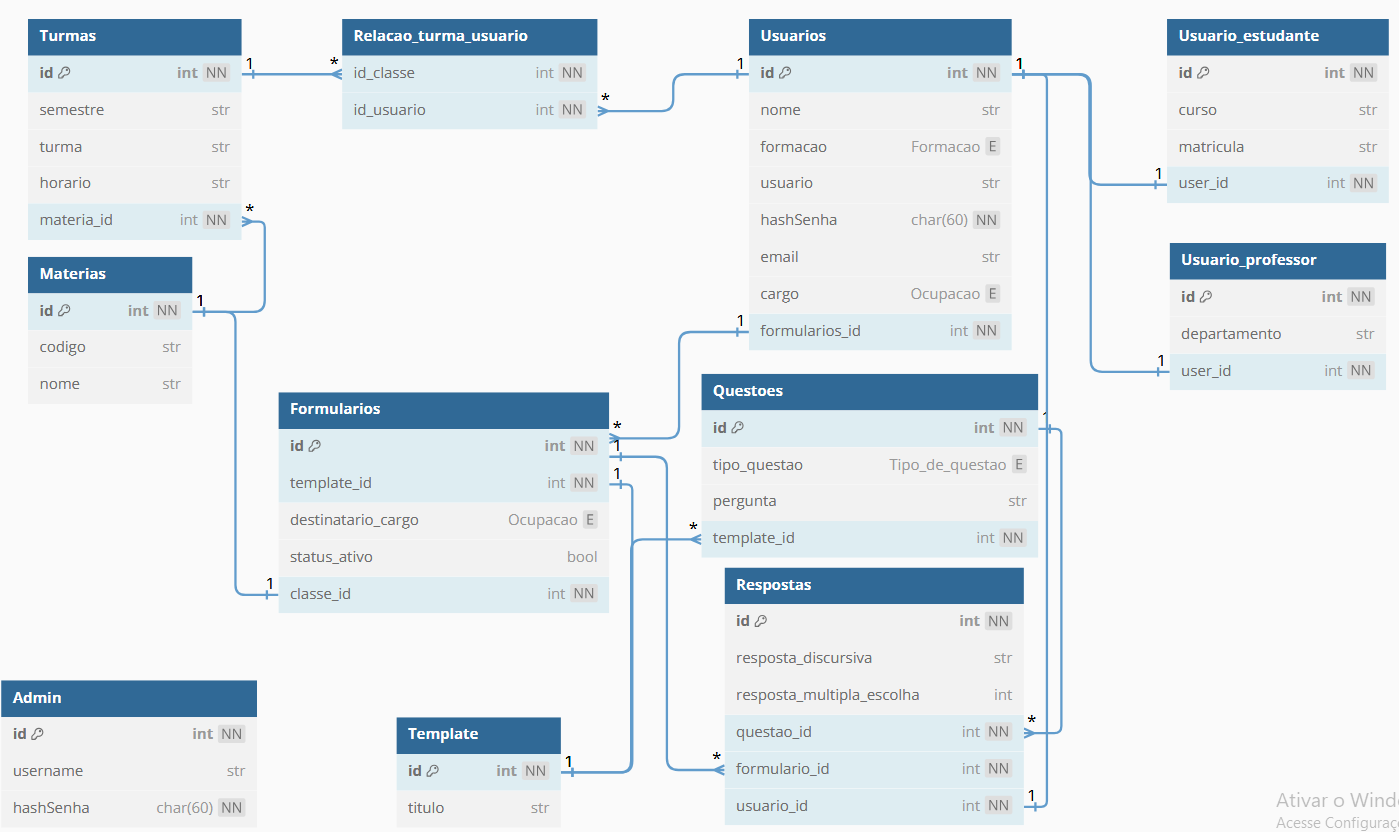
\includegraphics[width=1\textwidth]{./Imagens/Diagrama_de_Classes.png}

    \caption{Modelo Relacional UML da aplicação Camaar. \href{https://dbdiagram.io/d/Diagrama-BD-Eng-Software-6862ccc5f413ba350893b624}{Diagrama BD UML}}

    \label{fig:uml}

\end{figure}

\section*{Considerações Finais}

O modelo apresentado organiza de forma clara a estrutura do sistema \textbf{Camaar}, permitindo a gestão eficiente de formulários educacionais. Com entidades bem definidas, o sistema é escalável, de fácil manutenção e preparado para futuras extensões, como novos tipos de usuários, formatos de questões e geração de relatórios.
 
\end{document}

 